\section{La realidad, <<The Electronic WasteLand>>}

Tal y como se ha visto a lo largo del artículo, los gobiernos aparentemente están legislando para resolver el problema de la e-basura aunque ya se ha visto que la legislación es muy laxa, debido a los altos costes de los procedimientos de reciclaje y de reutilización y los grandes lobbys de compañías fabricantes que no quieren incurrir en los mismos. Iniciativas para crear estándares que faciliten este proceso también se han iniciado pero todavía no han concretado en nada realmente útil y provechoso.

Al amparo de todo esto, han surgido un gran número de compañías, cuyo negocio es el reciclaje de la e-basura, atraídos por los impuestos y subvenciones que los gobiernos han establecido para la realización de estos servicios. 

Están también surgiendo empresas de innovación tecnológica que están tratando de industrializar y simplificar el proceso para realizarlo más eficientemente y de forma más económica.

Sin embargo, todo esto, queda en un conjunto de buenos deseos y buenas intenciones. Las estadísticas oficiales muestran que solo un 33\% de la e-basura pasa por las plantas de reciclado y tal y como se ha podido ver en varios reportajes de investigación, como el reportaje de la cadena CBS News, <<The Electronic WasteLand>>, \cite{wasteland}, la realidad detrás de estas empresas de reciclaje no siempre es lo que esperamos.

En este reportaje se muestra una compañía especializada en reciclaje de e-basura a la que ciudadanos de los Estados Unidos entregan sus viejos dispositivos pensando que van a ser reciclados. De hecho existen grandes colas de espera para poder entregar los dispositivos.

\begin{figure}[H]
\begin{center}
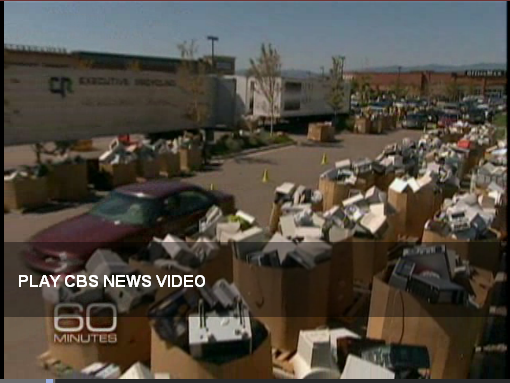
\includegraphics[width=0.5\textwidth]{img/screen1}
\caption{Screenshot reportaje CBS News - The Electronic WasteLand}
\end{center}
\end{figure}

Dentro de la compañía se observa un trasiego muy importante de contenedores y camiones. Los autores del reportaje deciden investigar y observan que en los camiones viajan muchos materiales que en principio debían ser reciclados en la planta. Estos materiales son trasladados en barco a Hong Kong (República Independiente de China).

\begin{figure}[H]
\begin{center}
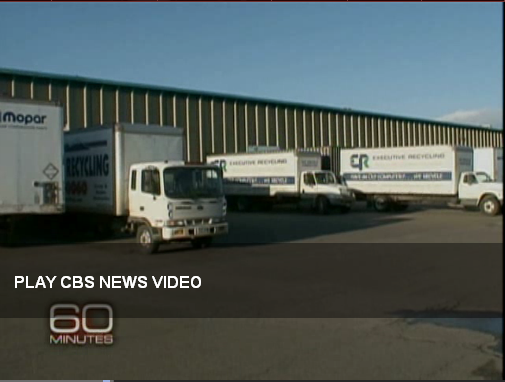
\includegraphics[width=0.4\textwidth]{img/screen2}
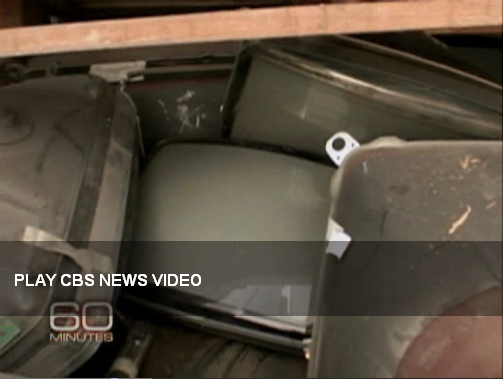
\includegraphics[width=0.4\textwidth]{img/screen3}
\caption{Screenshots reportaje CBS News - The Electronic WasteLand}
\end{center}
\end{figure}

\begin{figure}[H]
\begin{center}
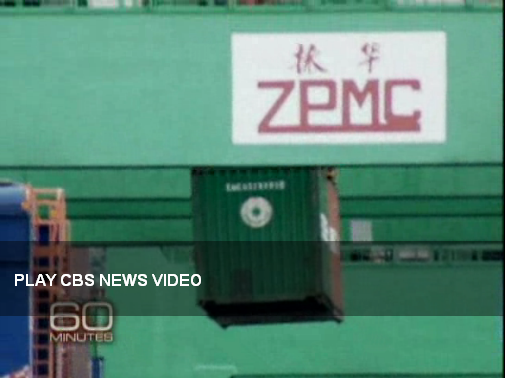
\includegraphics[width=0.4\textwidth]{img/screen4}
\caption{Screenshot reportaje CBS News - The Electronic WasteLand}
\end{center}
\end{figure}

Investigando en el interior del territorio chino se empieza a visualizar donde acaba realmente la e-basura. Acaba en vertederos ilegales donde la población china, en unas condiciones insalubres, revuelve en los mismos tratando de recuperar distintos materiales (sobre todo metales de distintas tipologías) para posteriormente venderlos. Al amparo de esta actividad, se construyen autenticas ciudades de gente cuyo labor permanente es rebuscar en estos amplios vertederos. Las poblaciones de estos territorios afrontan graves problemas de salud debido a la alta toxicidad de los distintos elementos que tratan y manipulan sin seguir las mínimas normas de seguridad. 

\begin{figure}[H]
\begin{center}
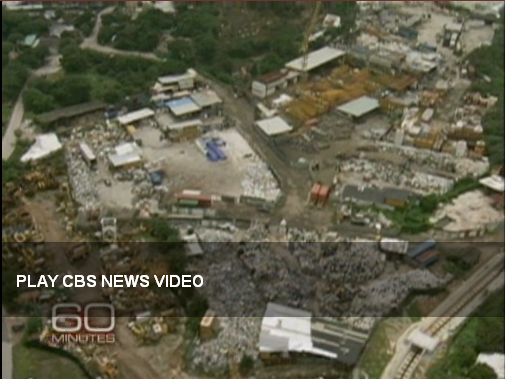
\includegraphics[width=0.4\textwidth]{img/screen5}
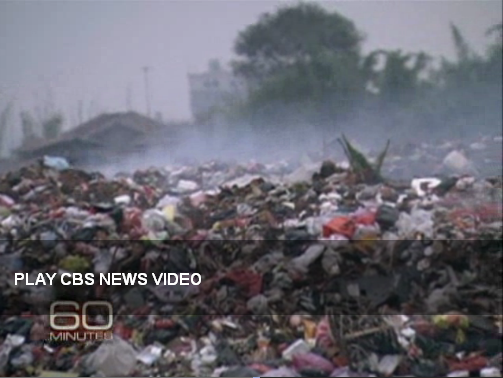
\includegraphics[width=0.4\textwidth]{img/screen6}
\caption{Screenshots reportaje CBS News - The Electronic WasteLand}
\end{center}
\end{figure}


Esta es la dura realidad de la e-basura que se repite a lo largo de varios países en vías de desarrollo o subdesarrollados. El mundo occidental traslada su basura a estos entornos en lugar de afrontar un proceso de reutilización y reciclaje a pesar de los beneficios que se pueden obtener del mismo, tal y como se detallan en \cite{reusing-silicon}.